%\documentclass[conference]{IEEEtran}
\documentclass{IEEEcsmag}
\IEEEoverridecommandlockouts
% The preceding line is only needed to identify funding in the first footnote. If that is unneeded, please comment it out.
%\usepackage{cite}
\usepackage{amsmath,amssymb,amsfonts}
\usepackage{algorithmic}
\usepackage{graphicx}
\usepackage{textcomp}
\usepackage{xcolor}
\usepackage[square,numbers,comma]{natbib}
\usepackage{booktabs}
\usepackage{listings}
\usepackage{amssymb}
\usepackage{array}
\usepackage{multirow}
\usepackage{multicol}
% ===== Dennis added ====
\usepackage{cancel}
\usepackage{hyperref}
\renewcommand*{\thesection}{\arabic{section}}
\usepackage{lipsum}
\usepackage[colorinlistoftodos]{todonotes}
\usepackage{soul}
%https://tex.stackexchange.com/questions/71162/reset-section-numbering-between-unnumbered-chapters
% ======== end ==========
\def\BibTeX{{\rm B\kern-.05em{\sc i\kern-.025em b}\kern-.08em
    T\kern-.1667em\lower.7ex\hbox{E}\kern-.125emX}}
    
\newcommand{\IC}[1]{\textcolor{red}{\textit{IC: #1}}}
\newcommand{\red}[1]{\textcolor{red}{#1}} 

\usepackage{listings}
\usepackage{xcolor}

\definecolor{codegreen}{rgb}{0,0.6,0}
\definecolor{codegray}{rgb}{0.5,0.5,0.5}
\definecolor{codepurple}{rgb}{0.58,0,0.82}
\definecolor{backcolour}{rgb}{1,1,1}

\lstdefinestyle{mystyle}{
    backgroundcolor=\color{backcolour},   
    commentstyle=\color{codegreen},
    keywordstyle=\color{magenta},
    numberstyle=\tiny\color{codegray},
    stringstyle=\color{codepurple},
    basicstyle=\ttfamily\footnotesize,
    breakatwhitespace=false,         
    breaklines=true,                 
    captionpos=b,                    
    keepspaces=true,                 
    numbers=left,                    
    numbersep=5pt,                  
    showspaces=false,                
    showstringspaces=false,
    showtabs=false,                  
    tabsize=2
}

\lstset{style=mystyle}

\begin{document}

\title{Practices and Infrastructures for ML Systems -- An Interview Study in Finnish Organizations}

\author{\IEEEauthorblockN{Dennis Muiruri,
Lucy Ellen Lwakatare, Jukka K. Nurminen and
Tommi Mikkonen}
\IEEEauthorblockA{Department of Computer Science,
University of Helsinki\\
Email: dennis.muiruri@helsinki.fi, lucy.lwakatare@helsinki.fi, jukka.k.nurminen@helsinki.fi,  tommi.j.mikkonen@jyu.fi 
}
}

\begin{abstract}
Practices and infrastructures for developing and maintaining machine learning (ML) enabled software systems are often reported by prominent and experienced data-driven organizations. However, little is known about the state of practice in other types of organizations. Using interviews, we investigate practices and toolchains for ML-enabled systems from sixteen organizations across various domains in Finland. Our study observes a high adoption of some well-established AI engineering practices and tools, especially in conducting ML model experiments. However, the field still needs to define and establish practices and tools for the end-to-end testing of ML systems and monitoring the ML models in production.
\end{abstract}

\maketitle

\section{\textbf{Introduction}}
\label{sec: introduction}
Today, artificial intelligence (AI) techniques are incorporated in many real-world software systems and services. However, research on the development, deployment and maintenance of AI-enabled systems in industrial settings report this to be a challenging task \cite{Sculley2015, Lwakatare2019}. Large companies, like Google \cite{Baylor2017} and Facebook \cite{Hazelwood2018Facebook}, often report their development and infrastructure practices for AI solutions that are useful for learning. However, many organizations are yet to adopt and tailor the suggested development practices and infrastructures to narrow the gap from mere prototyping to deploying to production AI solutions \cite{Serban2020Practices}. 

Machine learning (ML) is a subset of AI and its techniques involve the use of high-quality data. In ML logic is not explicitly programmed but is rather learned from data. The development of industrial ML-enabled software systems involves ML pipelines that consist of several interlocking steps. To support the different steps, end-to-end in one environment, ML platforms like TensorFlow Extended (TFX) \cite{Baylor2017}, have been proposed to ensure increased automation across the steps.

Since industrial ML pipelines can be complex, it is important to gain an understanding of their characteristics. In a large data-intensive organization, like Google, all 3000 ML pipelines comprising of over 450,000 trained ML models continuously update the models at least seven times a day \cite{Doris2021MLPipelines}. %A one-off ML pipeline is typically initiated to produce trained ML models ‘on-demand’, whereas a continuous ML pipeline continuously updates the models in production \cite{Baylor2019}. 
The need to support regular model training and updates in production is a common requirement in most industrial ML-enabled systems because, often, data is constantly being generated and the performance of models can deteriorate overtime \cite{Sculley2015}.

Most empirical literature presents development and maintenance practices of ML-enabled systems from the perspective of a single, often large and experienced online organization. In contrast, we aim to provide empirical evidence of the practices and infrastructure setups across a diverse set of companies in various domains. Through interviews, this study investigated ML workflow practices and toolchains used in the development, deployment, and maintenance of ML-enabled systems in selected multiple organizations in Finland. Our main contributions include:
\begin{itemize}
    \item Empirical evidence of common practices in ML workflows (Section \ref{sec:practices})
    \item Tool adoption in ML pipelines (Section \ref{sec:tools}) and areas to address in future research (Section \ref{sec:discussion})
    %\item %Remaining challenges (Section \ref{sec:challenges}) and 
    
\end{itemize}

%The rest of the paper is organized as follows. Section \ref{sec:background} presents background and related work within the scope of this research. The research approach of the study is presented in Section \ref{sec: methodology} . The study results are presented in Section \ref{sec:findings} and discussed in Section \ref{sec:discussion}. Finally, Section \ref{sec:conclusion} concludes the paper.

%Few studies have sought to specify the best engineering practices and their effects across multiple organisations rather than focusing on a particular organization \cite{Serban2020Practices}.


\section{\textbf{Background and related work}}
\label{sec:background}
%This section presents empirical studies on development, deployment, and maintenance of ML-enabled systems. The focus is on works that describe the characteristics of industrial ML workflows and pipelines for ML systems.
%\red{should we add a section intro here? In other sections there is something, but here not?}

\subsection{Software engineering for machine learning}
Adaptation of well-established software engineering (SE) methods and approaches in ML systems have been reported to be crucial \cite{Amershi2019}. This perspective emphasizes important aspects of ML model development and operations in production, such as data management and serving infrastructure \cite{Sculley2015}. Earlier studies observed that companies with fewer years of experience in deploying to production ML components adopt less of the identified SE best practices in ML \cite{Serban2020Practices}. In addition, the companies are also reported to face different SE challenges at different evolution stages of deploying ML components in software-intensive systems (experimentation \& prototyping, non-critical deployment, critical deployment, cascading deployment, and autonomous ML components) \cite{Lwakatare2019}.
%A taxonomy is proposed and used to map the SE challenges at each evolution stage (experimentation & prototyping, non-critical deployment, critical deployment, cascading deployment, and autonomous ML components). }

%Best SE practices in ML have been identified and their adoption in the industry surveyed %\st{in}
%\cite{Serban2020Practices}. 

The identified best SE practices in ML include those pertaining to data (e.g., employing sanity checks for all external data sources), training (e.g., use versioning for data, model, configurations and training scripts), coding (e.g., using continuous integration, deployment (e.g., enabling shadow deployment), team (e.g., collaborating with multidisciplinary team members), and governance (enforcing fairness and privacy) \cite{Serban2020Practices}. According to the authors \cite{Serban2020Practices}, the least adopted practices --  related to feature management, writing tests, shadow deployment and automated hyper-parameter optimization -- require effort, knowledge and tool support. 

%This interview study provides some validation and in-depth interpretation to the survey findings related to the adoption of \textcolor{green}{these} practices \cite{Serban2020Practices}.  

\subsection{ML workflow and pipelines}

ML workflows describe different tasks which are performed in order to develop, deploy and operate ML models in production \cite{Amershi2019}. ML pipelines are used to express complex input/output relationship between 
different tasks/operators of an automated ML workflow \cite{Doris2021MLPipelines}. Generally, ML pipelines plug together several tools to automate ML workflows \cite{Hummer2019IBM}.

A typical ML workflow life-cycle includes model requirements, data collection, data cleaning, data labelling, feature engineering, model training, model evaluation, model deployment and model monitoring \cite{Amershi2019}. Studies show that end-to-end automation of ML workflows improves both the development time and rate of deploying ML models \cite{Hummer2019IBM,Doris2021MLPipelines}. Furthermore, it allows organizations to automate orchestration of workflows steps, track and reproduce the outputs of a ML workflow, and reuse common steps of the workflow across multiple ML systems \cite{Baylor2017, Hummer2019IBM}. %In addition to ML workflow components, MLOps tools provide utilities to manage pipeline execution and schedule training jobs.

Few studies report in detail the characteristics of ML pipelines in terms of their components, and architectures \cite{Hummer2019IBM,Doris2021MLPipelines}. Different from our qualitative analysis, Xin et al \cite{Doris2021MLPipelines} quantitatively analysed over 3000 ML pipelines at Google and presented their high-level characteristic in terms of pipeline lifespan, complexity, and resource consumption. For the complexity of ML pipelines, the authors analyzed typical input data shape, feature transformation and model diversity. Model diversity showed that a large portion was neural networks (NN) (64\%) and model type and architecture influence the characteristics of the resulting ML pipelines. %\textcolor{red}{\st{ML pipelines due as pipeline steps can be different since the choice of model type and architecture has an influence on ML pipeline steps}}. 
From the study, the authors \cite{Doris2021MLPipelines} identified data management-related areas as key for optimizing ML pipelines. %\st{From the study, the authors \cite{Doris2021MLPipelines} identified areas for optimizing the ML pipelines, that were mostly related to data management}.

%Data infrastructure is critical when developing an ML-enabled system because it influences the performance, fairness, robustness, safety, and scalability of the system. Developers of ML-enabled systems are often reported to struggle most with data acquisition and management \cite{makinen2021needs}. The latter includes spending a significant portion of time to analyse raw data and handle data errors, such as differences in data distribution at training and serving (training-serving skew). To ensure high-quality data in ML pipelines, data validation tools, such as TFX Data Validation \cite{Baylor2017} are proposed for detecting data errors. These have focus on the data cleaning phase, and there is a need for extension in both upstream (data creation) and downstream (live data after deployment) \cite{Sambasivan2021}.




%Environment abstractions
%The operationalization of ML solutions often involve moving different assets (data, model, application) between different environments up until deployment to production environment. Typically, ML model is developed in an iterative manner in a local environment (e.g., using Jupyter Notebook) with a sample of offline dataset. For production deployment, ML model must be integrated with data infrastructure in order to use live training data as well as with the serving infrastructure in order to 

%Once, implemented ML model can be moved to staging/test environment before deployment to production. Despite the trend of training ML models on the cloud where there is abundant GPU-backed VMs and containers, cite{Hummer2019IBM} noticed a significant number of AI systems use on-premise servers, dedicated clusters, edge devices or a combination and this heterogeneity introduce a number of challenges. 

% Metadata management
%Tracking metadata of AI artifacts across the lifecycle is important for reproduciability of ML experiments. 


% Monitoring




%


\section{\textbf{Methodology}}
\label{sec: methodology}
% Insert table with summary of projects
%% Table generated by Excel2LaTeX from sheet 'practitioners_projects'
%DIF < \begin{table}[t]
%DIF >  \begin{table}[t]
%  \centering
%  \caption{A summary of interviewee roles}
%     \begin{tabular}{l l}
%     \toprule
%     \textbf{Roles} & \textbf{Role Type} \\
%     \toprule
%     Chief Machine Learning Engineer & Technical \\
%     Chief Scientific Officer & Technical \\
%     Head of Natural Language Understanding & Technical \\
%     Machine Learning Engineer (Founder) & Technical \\
%     Solution Architect & Technical \\
%     Director & Manager \\
%     Chief Machine Learning Engineer & Technical \\
%     Data Science Manager & Manager \\
%     Innovation Architect  & Technical \\
%     Chief Architect  & Technical \\
%     Data Scientist & Technical \\
%     AI Specialist & Technical \\
%     Director of Consulting & Manager \\
%     Data Scientist & Technical \\
%     Data Scientist & Technical \\
%     Machine Learning Engineer & Technical \\
%     Computational Biologist & Technical \\
%     Data Scientist & Technical \\
%     Site Lead & Manager \\
%     AI Engineer & Technical \\
%     Chief Data Architect & Manager \\
%     Principle Data Scientist & Manager \\
%     Data Scientist & Technical \\
%     \hline
%     \end{tabular}%
%  \label{tab:practioners}%
%DIF < \end{table}%
%DIF >  \end{table}%

\begin{table*}[h!]
  \centering
  \caption{Summary of participants demographics}
    \begin{tabular}{lp{12cm} }
    \toprule
    \textbf{Type} & \textbf{Count} \\
    \toprule
    Role & Chief Machine Learning Engineer (2), Chief Scientific Officer, Head of Natural Language Understanding,  Machine Learning Engineer (Founder), Solution Architect, Director, Data Science Manager, Chief Architect, Data Scientist (5), AI Specialist, Director of Consulting, Machine Learning Engineer, Computational Biologist, Site Lead, AI Engineer, Chief Data Architect, Principle Data Scientist \\
    \midrule

    Org. Size & Small-Medium sized (5),  Large size (11)\\
    \midrule

    Org. Business Focus & Product (6), Services (4), Consultancy (4) , Product \& services (1), Public services (1)\\
    \midrule

    Sector & Healthcare (1), Banking \& Financial services (3), Public agency (1), Pharmaceutical (1), Gaming (1), Paper \& Forest (1), Real-estate (1), Electricity (1), Media (1), Engineering and service (1), Computer software (2)\\
    \midrule

    ML Type & Computer vision (5), Speech recognition (2), MLOps (4), Analytics (5), Natural Language Processing (2), Recommendation systems (1)\\
    \bottomrule

    \end{tabular}%
  \label{tab:practioners}%
\end{table*}%





\DIFdelbegin \DIFdel{We conducted an }\DIFdelend \DIFaddbegin \DIFadd{An }\DIFaddend exploratory multiple-case study \cite{Runeson2008} \DIFaddbegin \DIFadd{was conducted }\DIFaddend between March and August 2021. 
%The research data was primarily collected through semi-structured interviews ~\cite{myers2007qualitative, Runeson2008}. 
The main research questions (RQ) \DIFdelbegin \DIFdel{of our study were}\DIFdelend \DIFaddbegin \DIFadd{include}\DIFaddend :
\begin{itemize}
    \item RQ1. What practices are applied in the development, deployment and maintenance of industrial ML-enabled software systems?
    \item RQ2. What tools are used to support the development, deployment and maintenance of industrial ML-enabled software systems?
   % \item RQ3. What challenges remain to be addressed in the development, deployment and maintenance of industrial ML-enabled software systems?
\end{itemize}
%involving two interviewers and one or multiple interviewees. 

\subsection{Research design and case selection}
The main goal of our study is to understand the state-of-practice of ML-enabled systems' development and toolchain within the Finnish context. In this study, a case (Table \ref{tab:data_source_storage_mlframeworks}) is an organization in Finland with experience in developing, deploying and maintaining ML-enabled software systems. The main criterion for case selection is that the ML-enabled software system needs to be operational in a production environment. %As such, our primary focus is to gather information on the whole system development life cycle from experiment to operations.

%Based on the study objective, at the initial phase, 
We first identified relevant practitioners from different organizations to take part in the study and adapted an interview guide used in an earlier study \cite{Lwakatare2019}. \DIFaddbegin \DIFadd{For the current study, we modified questions under the project background and characteristics section of the interview guide in order to only inquire about operational ML systems rather than practitioners' general experience in ML projects. This was done to exclude ML systems that are in experimental or prototyping stage because they are observed not only to employ immature practices and toolchains but also face different SE challenges \mbox{%DIFAUXCMD
\cite{Lwakatare2019}}\hskip0pt%DIFAUXCMD
. In addition, we added new questions that asked about the infrastructure and tools used for the different activities of ML system development and operations. }\DIFaddend The identified practitioners (or their organizations) were primarily known to be working on ML solutions by the researchers and others were gathered from LinkedIn. %\footnote{https://www.linkedin.com/}  LinkedIn targets were identified based on their indication of holding a position that we considered to be related to ML. 

We reached out to 37 organizations via e-mail out of which 16 agreed to participate in the study. %The e-mails also detailed the study objectives, scope and data collection procedure. 
Generally, practitioners were free to choose whether (and who) to participate in the study, but researchers purposefully ensured that the organizations were varied in terms of sector and size. 

Interviewed practitioners had varying roles: Chief Machine Learning Engineer (2), Chief Scientific Officer, Head of Natural Language Understanding,  Machine Learning Engineer (Founder), Solution Architect(2), Director, Data Science Manager, Chief Architect, Data Scientist (5), AI Specialist, Director of Consulting, Machine Learning Engineer, Computational Biologist, AI Engineer, Chief Data Architect, Principle Data Scientist.
%The average length of experience in the indicated role is 2.2 years while the minimum and maximum are 4 months and 8.6 years respectively. 
%Following the description of the roles and organisational structure given by interviewees, we grouped the interviewees to hold either a technical or managerial role, from this perspective, seventeen (74\%) interviewees held technical roles while six (26\%) held management or leadership type of roles. One of the technical interviewees was also a founder of the company. 
Academically, ten (43\%) practitioners hold a PhD degree, ten (43\%) hold a Master's degree and two (9\%) hold a Bachelor's degree. %and one (4\%) practitioner had selectively taken courses. %but did not complete the studies
% A table to show practitioners' profile
%% Table generated by Excel2LaTeX from sheet 'practitioners_projects'
%DIF < \begin{table}[t]
%DIF >  \begin{table}[t]
%  \centering
%  \caption{A summary of interviewee roles}
%     \begin{tabular}{l l}
%     \toprule
%     \textbf{Roles} & \textbf{Role Type} \\
%     \toprule
%     Chief Machine Learning Engineer & Technical \\
%     Chief Scientific Officer & Technical \\
%     Head of Natural Language Understanding & Technical \\
%     Machine Learning Engineer (Founder) & Technical \\
%     Solution Architect & Technical \\
%     Director & Manager \\
%     Chief Machine Learning Engineer & Technical \\
%     Data Science Manager & Manager \\
%     Innovation Architect  & Technical \\
%     Chief Architect  & Technical \\
%     Data Scientist & Technical \\
%     AI Specialist & Technical \\
%     Director of Consulting & Manager \\
%     Data Scientist & Technical \\
%     Data Scientist & Technical \\
%     Machine Learning Engineer & Technical \\
%     Computational Biologist & Technical \\
%     Data Scientist & Technical \\
%     Site Lead & Manager \\
%     AI Engineer & Technical \\
%     Chief Data Architect & Manager \\
%     Principle Data Scientist & Manager \\
%     Data Scientist & Technical \\
%     \hline
%     \end{tabular}%
%  \label{tab:practioners}%
%DIF < \end{table}%
%DIF >  \end{table}%

\begin{table*}[h!]
  \centering
  \caption{Summary of participants demographics}
    \begin{tabular}{lp{12cm} }
    \toprule
    \textbf{Type} & \textbf{Count} \\
    \toprule
    Role & Chief Machine Learning Engineer (2), Chief Scientific Officer, Head of Natural Language Understanding,  Machine Learning Engineer (Founder), Solution Architect, Director, Data Science Manager, Chief Architect, Data Scientist (5), AI Specialist, Director of Consulting, Machine Learning Engineer, Computational Biologist, Site Lead, AI Engineer, Chief Data Architect, Principle Data Scientist \\
    \midrule

    Org. Size & Small-Medium sized (5),  Large size (11)\\
    \midrule

    Org. Business Focus & Product (6), Services (4), Consultancy (4) , Product \& services (1), Public services (1)\\
    \midrule

    Sector & Healthcare (1), Banking \& Financial services (3), Public agency (1), Pharmaceutical (1), Gaming (1), Paper \& Forest (1), Real-estate (1), Electricity (1), Media (1), Engineering and service (1), Computer software (2)\\
    \midrule

    ML Type & Computer vision (5), Speech recognition (2), MLOps (4), Analytics (5), Natural Language Processing (2), Recommendation systems (1)\\
    \bottomrule

    \end{tabular}%
  \label{tab:practioners}%
\end{table*}%




Ten cases are large organizations and five constitute small or medium-sized organizations with revenues below €50 million based on 2020 financial reports\DIFdelbegin \DIFdel{(https://bit.ly/3BtbFgN)}\DIFdelend .
%Most of the organizations had a specific focus of either products (7 of 16) or services (4 of 16), and few were consultancies (3 of 16). As listed in Table~\ref{tab:practioners}, the types of ML solutions worked on included: computer vision (3), automatic speech recognition (ASR) (2), general ML operations (2), analytics platforms with ML features (4), data analysis (1), natural language processing (NLP) (2), data lake (1), and recommendation systems (1). 

\subsection{Data collection}

Research data was primarily collected through semi-structured interviews conducted by two researchers. A total of 23 practitioners from the 16 organizations were interviewed between 24$^{th}$ March and 27$^{th}$ April 2021. All interviews were conducted virtually due to COVID-19. Each interview session took on average 80 minutes. 

During the interview session, the researchers presented details of the study and requested consent to record the interview. One researcher asked the question outlined in the interview guide that contained five broad categories: data management, model training, model deployment, model monitoring and general challenges. The interview guide was not strictly followed to allow probing questions depending on the interviewees' responses and their experience with the topic. All recorded interviews were automatically transcribed using Otter.ai and errors in the transcriptions were manually corrected by the researchers.  %An example of a topic, question and sub-question from our interview guide is shown in Table~\ref{tab:sample_questions}.

% Table: Interview guide extract
% Interview guide extract
%\begin{table*}[t]
%  \centering
%  \caption{An example of a topic, main question and a follow up question}
%    \begin{tabular}{ll}
%    \toprule
%    \multicolumn{1}{l}{\textbf{Topic}} &
%      Project background and characteristics \\
%    Question &
%      What type of machine learning based system are you currently working on or consulting about? \\
%    Sub-question &
%How would you classify the area of ML/AI you are involved in? for example NLP, Speech, Computer vision etc.\\
%    \hline
%    \end{tabular}%
%  \label{tab:sample_questions}%
%\end{table*}%


\subsection{Data analysis}
Analysis of the interview transcripts mainly consisted of two coding steps and a session to discuss and harmonize the codes \cite{Runeson2008}. A deductive approach formed the first stage of our coding process in which main themes informed by the structure of our interviews were outlined. %This facilitated a unified structure and terminology in the analysis. 
The themes were constituted high-level codes organized into six groups: role and responsibility, organisation, ML usecase, Practices, Challenges and Tools. The actual coding of data was done in an iterative manner using both deductive and inductive \cite{Runeson2008} approaches within each group and applied broadly at a paragraph or statement level. The sub-groups were further refined during researcher meetings. 
%Our study had one interviewee per organization and neither did we prescribe the type of roles to be interviewed. As a result, we observe that interviewees had deeper insight into subject matters that fall within their current role especially in larger organizations characterised by dedicated teams in different aspects of the pipeline. In smaller case companies, interviewees had a broader perspective of the entire pipeline activities as team meetings and high-level development decisions often involved everyone in the organization. This may affect generalizability of our results.



%\section{Overview of the Cases}
%\label{sec: study_data}
%% Insert table with summary of projects
% Table generated by Excel2LaTeX from sheet 'practitioners_projects'
%DIF < \begin{table}[t]
%DIF >  \begin{table}[t]
%  \centering
%  \caption{A summary of interviewee roles}
%     \begin{tabular}{l l}
%     \toprule
%     \textbf{Roles} & \textbf{Role Type} \\
%     \toprule
%     Chief Machine Learning Engineer & Technical \\
%     Chief Scientific Officer & Technical \\
%     Head of Natural Language Understanding & Technical \\
%     Machine Learning Engineer (Founder) & Technical \\
%     Solution Architect & Technical \\
%     Director & Manager \\
%     Chief Machine Learning Engineer & Technical \\
%     Data Science Manager & Manager \\
%     Innovation Architect  & Technical \\
%     Chief Architect  & Technical \\
%     Data Scientist & Technical \\
%     AI Specialist & Technical \\
%     Director of Consulting & Manager \\
%     Data Scientist & Technical \\
%     Data Scientist & Technical \\
%     Machine Learning Engineer & Technical \\
%     Computational Biologist & Technical \\
%     Data Scientist & Technical \\
%     Site Lead & Manager \\
%     AI Engineer & Technical \\
%     Chief Data Architect & Manager \\
%     Principle Data Scientist & Manager \\
%     Data Scientist & Technical \\
%     \hline
%     \end{tabular}%
%  \label{tab:practioners}%
%DIF < \end{table}%
%DIF >  \end{table}%

\begin{table*}[h!]
  \centering
  \caption{Summary of participants demographics}
    \begin{tabular}{lp{12cm} }
    \toprule
    \textbf{Type} & \textbf{Count} \\
    \toprule
    Role & Chief Machine Learning Engineer (2), Chief Scientific Officer, Head of Natural Language Understanding,  Machine Learning Engineer (Founder), Solution Architect, Director, Data Science Manager, Chief Architect, Data Scientist (5), AI Specialist, Director of Consulting, Machine Learning Engineer, Computational Biologist, Site Lead, AI Engineer, Chief Data Architect, Principle Data Scientist \\
    \midrule

    Org. Size & Small-Medium sized (5),  Large size (11)\\
    \midrule

    Org. Business Focus & Product (6), Services (4), Consultancy (4) , Product \& services (1), Public services (1)\\
    \midrule

    Sector & Healthcare (1), Banking \& Financial services (3), Public agency (1), Pharmaceutical (1), Gaming (1), Paper \& Forest (1), Real-estate (1), Electricity (1), Media (1), Engineering and service (1), Computer software (2)\\
    \midrule

    ML Type & Computer vision (5), Speech recognition (2), MLOps (4), Analytics (5), Natural Language Processing (2), Recommendation systems (1)\\
    \bottomrule

    \end{tabular}%
  \label{tab:practioners}%
\end{table*}%





%This section provides a high-level overview of the studied cases. Our sample cases are composed of companies domiciled in Finland. 
%, practitioners and projects that we analyzed in this study. 
%Our study aimed to capture views from varying companies operating across different sectors. We focused on selecting companies with already deployed ML based solutions, such teams were considered to have the required experiences in managing machine learning solutions across their life cycle.
%63\% (10 of 16) of these companies are considerably large organizations with revenues ranging between €151,6 million and €49 billion based on 2020 financial reports\footnote{https://www.asiakastieto.fi/web/en/frontpage.html}. 31\% (5 of 16) were small or medium sized organizations with revenues below €50 million while one organisation 6\% is a public agency. The industrial sector differed amongst the organizations. While most organizations had a specific focus of either products (7 of 16) or services (4 of 16), there were few consultancies (3 of 16) that rendered varied contracted customer projects. 

%At the onset of the interviews, we requested interviewees to select a single anchoring project for the discussion whenever the company had multiple projects related to machine learning. A wide range of machine learning related projects were presented during the interviews, we summarize the project topics as shown in Table~\ref{tab:projects}\footnote{\textcolor{red}{Company column to be removed later}}. In summary, the ML projects were related to computer vision (3), speech recognition (2), general ML operations (2), analytics platforms with ML features (4), data analysis (1), natural language processing (2), data lakes (1) and recommendation systems (1).

%The ID column presents arbitrary IDs assigned to the company/project for reference purposes. The project column presents a given project's machine learning focus area and the context column aims to provide the problem being solved using the machine learning. Some of the ML topics appeared multiple times but the context of the project was often different.

%Based on reported revenues, we categorised the sample of companies into three groups: five (31\%)  SMEs\footnote{https://ec.europa.eu/growth/smes/sme-definition_en}, that is companies with revenues below €50 million, ten (63\%) large enterprises with revenues ranging between €151,6 million and €49 billion and one (6\%) public agency. The business profiles of these companies can be categorised as three (19\%) consulting companies, seven (44\%) product based companies, four (25\%) service companies, one (6\%) company offers a mix of products \& services and one (6\%) is a public service agency.

%\begin{figure}[h!]
%    \centering 
%    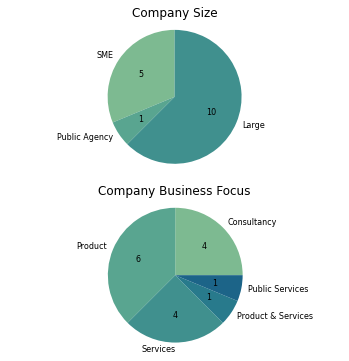
\includegraphics[width=0.5\textwidth]{images/company_views_vertical.png}
%    \caption{Descriptive data about companies involved in the study}
% \label{fig:company_data}
%\end{figure}





% \section{Findings}
% \label{sec:findings}




% ====== Research Question 1 =======

\section{\textbf{Practices in ML workflow (RQ1)}}
\label{sec:practices}


% Data Management
% Summary context, data collection, storage platforms
%% % Table summary of data collection, storage and ML frameworks
%% \begin{table}[t]
%%   \centering
%%   \caption{Summary of data sources and storage platforms}
%%   \begin{tabular}{clll}
%%     \hline
%%     Case & Data Source & Storage Solution & ML-Framework & ML-Category \\
%%     \hline
%%     A & Camera & Google cloud & Tensorflow & DL \\
%%     B & End users & AWS Tensorflow & DL \\
%%     C & End users & On-premise & Tensorflow, PyTorch, OpenCV & DL \\
%%     D & End users & Google cloud & Kaldi ASR framework  & DL \\
%%     E & Open source, End users & Google cloud & PyTorch & DL \\
%%     F & Camera & - & Tensorflow (Keras) and other frameworks & DL \\
%%     G & Trading systems & AWS & Tensorflow, Scikit-Learn & DL and Non-DL \\
%%     H & End users and internal systems & AWS & Scikit-Learn, XGBoost, Heuristics & Non-DL \\
%%     I & Sensor  and Technicians & AWS & Spark Analytics, Heuristics/Rules & Non-DL \\
%%     J & Sensor & Azure Cloud & - & Non-DL \\
%%     K & Meters & Azure Cloud & Scikit-learn, XGBoost & Non-DL \\
%%     L & Medical Device,  Genome Sequence & Azure Cloud & R & Non-DL \\
%%     M & System users & Azure Cloud & PyTorch, Scikit-learn (Classification) & Non-DL \\
%%     N & System users & AWS & Watson(IBM), Tensorflow, R & DL \\
%%     O & System users & Azure Cloud & - & Non-DL \\
%%     P & System users & AWS & Scikit-learn, Tensorflow(Keras), fastText & Non-DL \\
%%     \hline
%%     \end{tabular}%
%%   \label{tab:data_source_storage_mlframeworks}%
%% \end{table}%


% Table summary of data collection, storage and ML frameworks
%DIF > \begin{table*}[t]
%DIF >   \centering
%DIF >   \caption{Summary of ML usecase, frameworks, data sources and storage platforms across cases. (*of the ML usecase)}
%DIF >   \begin{tabular}{p{0,5cm}p{3,1cm}p{2cm}p{2,7cm}p{1,6cm}p{2,7cm}}
%DIF >     \toprule
%DIF >     \textbf{Case} & \textbf{ML usecase (Type)} & \textbf{Domain*} &\textbf{Data Source} & \textbf{Storage} & \textbf{ML-Framework} \\
%DIF >     \toprule \\
%DIF >     A & Object Detection (NN) & IoT & Camera & Google Cloud & Tensorflow \\
%DIF >     B & Form data extraction  (NN) & Finance & Internal Systems & AWS & Tensorflow \\
%DIF >     C & Form data extraction (NN) & Public Services & Internal Systems & On-premise & Tensorflow, PyTorch \\
%DIF >     D & Transcription (NN) & Healthcare & Internal Systems & Google Cloud & Kaldi ASR framework \\
%DIF >     E & Speech based UI (NN) & E-Commerce & Open-source, End-users & Google Cloud & PyTorch \\
%DIF >     F & MLOps (NN, Non-NN) & IT Services & Camera  & - & Multiple frameworks \\
%DIF >     G & MLOps (NN, Non-NN)  & Energy & Internal systems & AWS & Tensorflow, Scikit-Learn \\
%DIF >     H & Risk management (Non-NN) & Finance & Internal systems & AWS & Scikit-Learn, Heuristics \\
%DIF >     I & Predictive maintenance (Non-NN) & Engineering & Sensor and Technicians & AWS &  Spark Analytics, Heuristics/Rules \\
 %DIF >    J & Predictive maintenance (Non-NN) & Biochemicals & Sensor & Azure Cloud & - \\
%DIF >     K & Anomaly detection (Non-NN) & Real Estate & Meters & Azure Cloud & Scikit-learn, %XGBoost \\
    %DIF > L & Data analysis (Non-NN) & Pharmaceutical & Device,  Genome & Azure Cloud & R \\
    %DIF > M & Report/Document classification (Non-NN) & Healthcare & Internal systems & Azure Cloud & PyTorch, Scikit-learn (Classification) \\
%DIF >     N & Chatbots, Profiling (NN) & Finance & Internal systems & AWS & Watson(IBM), Tensorflow \\
%DIF >     O & ML pipeline automation (Non-NN) & IT services & Internal Systems & Azure Cloud & - \\
%DIF >     P & Marketing/campaign management (NN) & Media & Internal systems & AWS & Scikit-learn, Tensorflow, fastText \\
%DIF >     \hline
    \DIFaddbegin 


%DIF >     \end{tabular}%
%DIF >   \label{tab:data_source_storage_mlframeworks}
%DIF > \end{table*}% Add a role with multi column to add the text "caption"


%DIF > %%% with interviewees
%DIF > % Table summary of data collection, storage and ML frameworks
\DIFaddend \begin{table*}[t]
 \centering
  \caption{Summary of ML usecase, frameworks, data sources and storage platforms across cases. (*of the ML usecase)}
  \DIFdelbeginFL %DIFDELCMD < \begin{tabular}{p{0,5cm}p{3,4cm}p{2cm}p{2,7cm}p{1,6cm}p{2,7cm}}
%DIFDELCMD <     %%%
\DIFdelendFL \DIFaddbeginFL \begin{tabular}{p{0,4cm}p{2,1cm}p{2,8cm}p{1,8cm}p{2cm}p{1cm}p{2,3cm}}
    \DIFaddendFL \toprule
    \textbf{Case} & \DIFaddbeginFL \textbf{\DIFaddFL{Interviewee Role}} & \DIFaddendFL \textbf{ML usecase (Type)} & \textbf{Domain*} &\textbf{Data Source} & \textbf{Storage} & \textbf{ML-Framework} \\
    \toprule \\
    A & \DIFaddbeginFL \DIFaddFL{Chief ML Eng., Founder }& \DIFaddendFL Object Detection (NN) & IoT & Camera & \DIFdelbeginFL \DIFdelFL{Google Cloud }\DIFdelendFL \DIFaddbeginFL \DIFaddFL{GCP }\DIFaddendFL & Tensorflow \\
    B & \DIFaddbeginFL \DIFaddFL{Chief ML Eng. }& \DIFaddendFL Form data extraction  (NN) & Finance & Internal Systems & AWS & Tensorflow \\
    C & \DIFaddbeginFL \DIFaddFL{Chief architect }& \DIFaddendFL Form data extraction (NN) & Public Services & Internal Systems & On-premise & Tensorflow, PyTorch \\
    D & \DIFaddbeginFL \DIFaddFL{Chief scientific Officer }& \DIFaddendFL Transcription (NN) & Healthcare & Internal Systems & \DIFdelbeginFL \DIFdelFL{Google Cloud }\DIFdelendFL \DIFaddbeginFL \DIFaddFL{GCP }\DIFaddendFL & Kaldi ASR framework \\
    E & \DIFaddbeginFL \DIFaddFL{Head of NLU }& \DIFaddendFL Speech based UI (NN) & E-Commerce & Open-source, End-users & \DIFdelbeginFL \DIFdelFL{Google Cloud }\DIFdelendFL \DIFaddbeginFL \DIFaddFL{GCP }\DIFaddendFL & PyTorch \\
   F & \DIFaddbeginFL \DIFaddFL{ML Eng, Founder }& \DIFaddendFL MLOps (NN, Non-NN) & IT Services & Camera  & - & Multiple frameworks \\
    G & \DIFaddbeginFL \DIFaddFL{ML Eng. }& \DIFaddendFL MLOps (NN, Non-NN)  & Energy & Internal systems & AWS & Tensorflow, Scikit-Learn \\
    H & \DIFaddbeginFL \DIFaddFL{Solution Architect }& \DIFaddendFL Risk management (Non-NN) & Finance & Internal systems & AWS & Scikit-Learn, Heuristics \\
    I & \DIFaddbeginFL \DIFaddFL{Data Science Mgr }& \DIFaddendFL Predictive maintenance (Non-NN) & Engineering & Sensor and Technicians & AWS &  Spark Analytics, Heuristics/Rules \\
    J & \DIFaddbeginFL \DIFaddFL{Data Architect }& \DIFaddendFL Predictive maintenance (Non-NN) & Biochemicals & Sensor & \DIFdelbeginFL \DIFdelFL{Azure Cloud }\DIFdelendFL \DIFaddbeginFL \DIFaddFL{AC }\DIFaddendFL & - \\
    K & \DIFaddbeginFL & \DIFaddendFL Anomaly detection (Non-NN) & Real Estate & Meters & \DIFdelbeginFL \DIFdelFL{Azure Cloud }\DIFdelendFL \DIFaddbeginFL \DIFaddFL{AC }\DIFaddendFL & Scikit-learn, XGBoost \\
    L & \DIFaddbeginFL & \DIFaddendFL Data analysis (Non-NN) & Pharmaceutical & Device,  Genome & \DIFdelbeginFL \DIFdelFL{Azure Cloud }\DIFdelendFL \DIFaddbeginFL \DIFaddFL{AC }\DIFaddendFL & R \\
    M & \DIFaddbeginFL & \DIFaddendFL Report/Document classification (Non-NN) & Healthcare & Internal systems & \DIFdelbeginFL \DIFdelFL{Azure Cloud }\DIFdelendFL \DIFaddbeginFL \DIFaddFL{AC }\DIFaddendFL & PyTorch, Scikit-learn (Classification) \\
    N & \DIFaddbeginFL & \DIFaddendFL Chatbots, Profiling (NN) & Finance & Internal systems & AWS & Watson(IBM), Tensorflow \\
    O & \DIFaddbeginFL & \DIFaddendFL ML pipeline automation (Non-NN) & IT services & Internal Systems & \DIFdelbeginFL \DIFdelFL{Azure Cloud }\DIFdelendFL \DIFaddbeginFL \DIFaddFL{AC }\DIFaddendFL & - \\
    P &\DIFaddbeginFL & \DIFaddendFL Marketing/campaign management (NN) & Media & Internal systems & AWS & Scikit-learn, Tensorflow, fastText \\
    \hline
    \DIFaddbeginFL 

       
    \multicolumn{7}{l}{
    Organizations often use cloud storage providers with data centres  either in Finland, close proximity to Finland or within}\\

    \multicolumn{7}{l}{the European Union area following customer preferences or regulatory constraints. In certain cases, data is stored in private }\\

    \DIFaddendFL \end{tabular}%
  \DIFdelbeginFL %DIFDELCMD < \label{tab:data_source_storage_mlframeworks}%%%
\DIFdelendFL \DIFaddbeginFL \label{tab:data_source_storage_mlframeworks_interviewees}\DIFaddendFL %
\end{table*}%
\DIFaddbegin \DIFadd{This section presents common practices observed across the cases as summarized in Table~\ref{tab:practices_challenges}.
}\DIFaddend 

\subsection{Data management}
%DIF < Generally, data used to train the case ML systems is largely unstructured or semi-structured data, which in its basic form is composed of images/video, pdf files, text files, or genome sequencing data. In a few instances structured data is used to generate analytics with supporting ML based features. 

\underline{\emph{Data collection and storage}}
% Batch vs Real-time streams
\DIFdelbegin \DIFdel{typically begins either by }\DIFdelend \DIFaddbegin \DIFadd{are handled in various ways: }\DIFaddend batch loading data from internal systems, streaming from devices/sensors, extracting from \DIFdelbegin \DIFdel{other }\DIFdelend third-party vendors \DIFdelbegin \DIFdel{through APIs or from }\DIFdelend \DIFaddbegin \DIFadd{APIs or }\DIFaddend open-source repositories. The training data is then commonly stored in cloud platforms, as shown from data sources in Table ~\DIFdelbegin \DIFdel{\ref{tab:data_source_storage_mlframeworks}.
%DIF < or private infrastructure, a summary of the storage solutions  is presented in column "Storage Solution" of Table~\ref{tab:data_source_storage_mlframeworks}. Some organizations have multiple storage solutions, we only present the identified source of ML training data.
}\DIFdelend \DIFaddbegin \DIFadd{\ref{tab:data_source_storage_mlframeworks_interviewees}.
}\DIFaddend 

%DIF < Often this is due to data residency requirements where the data is required to reside in Finland. 
\DIFdelbegin \DIFdel{Organizations often use cloud storage providers with data centres either in Finland, close proximity to Finland or within the European Union geographic area following customer preferences or regulatory constraints. In very strict circumstances, data is stored in private infrastructure.
}%DIFDELCMD < 

%DIFDELCMD < %%%
\DIFdel{Additionally, low-level metrics , }\DIFdelend \DIFaddbegin \DIFadd{Low-level metrics }\DIFaddend such as IOPS (I/O Operations Per Second) \DIFdelbegin \DIFdel{, }\DIFdelend are considered when choosing a storage architecture\DIFdelbegin \DIFdel{as }\DIFdelend \DIFaddbegin \DIFadd{; }\DIFaddend data fetching can constitute a sizeable amount of the overall model training time. Case E uses \DIFaddbegin \DIFadd{a }\DIFaddend mounted discs solution instead of a network drive accessed via a web interface. %I/O bound process.

\underline{\emph{Data storage formats}} are \DIFdelbegin \DIFdel{also important architectural decisions when considering }\DIFdelend \DIFaddbegin \DIFadd{factored in when considering the }\DIFaddend scalability of data processing pipelines, \DIFdelbegin \DIFdel{portability of data }\DIFdelend \DIFaddbegin \DIFadd{data portability }\DIFaddend between computing environments, \DIFaddbegin \DIFadd{and }\DIFaddend support of different ML frameworks\DIFdelbegin \DIFdel{and programming languages. In this regard, two data storage formats are presented: the Apache Parquet (https://bit.ly/3kGFaVI) and the NetCDF (https://bit.ly/3zy287R) file formats.
}%DIFDELCMD < 

%DIFDELCMD < %%%
\DIFdelend \DIFaddbegin \DIFadd{. }\DIFaddend Case H uses Apache Parquet in \DIFdelbegin \DIFdel{favour }\DIFdelend \DIFaddbegin \DIFadd{favor }\DIFaddend of CSV (Comma Separated Values) or TSV (Tab Separated Values) file formats commonly used to store structured data for analytics purposes. Case G uses NetCDF \DIFdelbegin \DIFdel{as a solution }\DIFdelend to implement a generic data interface to abstract data across ML frameworks and computing platforms. 
\DIFdelbegin \DIFdel{Data scientists then ensure models can process NetCDF input and produce NetCDF output.
}\DIFdelend 

% \subsubsection{Data versioning}

\underline{\emph{Data discoverability and accessibility}}
\DIFdelbegin \DIFdel{affects the rate of experimentation and development of ML features. Discoverability tends to be a concern }\DIFdelend %DIF > affects the rate of experimentation and development of ML features. This 
\DIFaddbegin \DIFadd{is emphasized }\DIFaddend in setups that feature a data lake or where different \DIFdelbegin \DIFdel{types of data }\DIFdelend \DIFaddbegin \DIFadd{data types }\DIFaddend are collected. Case O describes a solution to this problem based on maintaining a \textit{data \DIFdelbegin \DIFdel{catalogue}\DIFdelend \DIFaddbegin \DIFadd{catalog}\DIFaddend } where data and its value are described. %This supports faster identification of data and its associated value. An alternative approach is to assign metadata to ingested data and the metadata can be made visible through custom tools.
\DIFdelbegin %DIFDELCMD < 

%DIFDELCMD < %%%
\DIFdel{Data access is a concern whenever an organization handles personal data or requires collaboration with third parties e.g. in consultancy settings. The process to grant data access can be lengthy and can result in data governance anti-patterns}\DIFdelend \DIFaddbegin \DIFadd{Data governance and related processes can limit the use and scope of data accessible for ML purposes}\DIFaddend .
%An example of such a data migration pattern involves an organization streaming data from its IoT devices to it's own cloud storage then a subset of the data is sent to a third party entity processor for cleaning or model training over an agreed interval. %https://www.linkedin.com/pulse/top-10-data-governance-anti-patterns-analytics-dave-wentzel

\underline{\emph{Data validation}}%DIF < Data ETL pipelines often include practices and mechanisms that ensure continuous collection or storage of clean data. Topical issues discussed relate to technical approaches, organisational set ups applied to collect good quality data and maintain data integrity.
techniques are commonly applied as a means of controlling data quality. However, data types influence the type of validation approaches \DIFdelbegin \DIFdel{applied. }\DIFdelend \DIFaddbegin \DIFadd{used. Validation of }\DIFaddend Image/video, speech\DIFaddbegin \DIFadd{, }\DIFaddend and text tend to require human actors supported by custom tools\DIFdelbegin \DIFdel{to validate and ensure data meets aspired quality thresholds. E.g, in an object detection setting, }\DIFdelend \DIFaddbegin \DIFadd{. For example, }\DIFaddend a human validator ensures that objects fall within the annotated bounding boxes \DIFdelbegin \DIFdel{. With speech , validation ensures that }\DIFdelend \DIFaddbegin \DIFadd{in an object detection setting. While a human speech validator ensures }\DIFaddend recorded utterances are coherent and consistent with corresponding text. Case D uses additional heuristics for detecting anomalies between generated texts and submitted utterances. Numerical data types \DIFdelbegin \DIFdel{normally easier to automatically validate .
%DIF < Other images can be validated by generating small image thumbnails which allow for a quick preview of the data or by using distribution graphs. 
}\DIFdelend \DIFaddbegin \DIFadd{usually are easier to validate automatically.
}\DIFaddend 

Data validation in Case O is done at a schema and data level. \DIFdelbegin \DIFdel{The schema is maintained by dedicated }\textit{\DIFdel{data stewards}} %DIFAUXCMD
\DIFdel{team that ensures the schemareflects the required data}\DIFdelend \DIFaddbegin \DIFadd{A dedicated data stewards maintain the schema}\DIFaddend . Delegating quality control ensures a team managing the data lake ingests data indiscriminately. When data is sourced from third-party vendors, the vendor is expected to maintain quality controls (Case P).
%DIF <  Control alarms are directed to this team whenever there is a quality breach such as incoming data not conforming to the defined schema or having erroneous data values.


\underline{\emph{Data integrity}}
controls ensure data is not changed unexpectedly. Case D and F apply hashing as part of data processing pipelines\DIFaddbegin \DIFadd{; }\DIFaddend this ensures training data is verifiable and traceable with respect to a model's lineage. Additionally, this practice ensures that attempts to overwrite data are flagged appropriately.

Generally, when hashing is not a suitable approach\DIFdelbegin \DIFdel{for example }\DIFdelend \DIFaddbegin \DIFadd{, for example, }\DIFaddend when dealing with image files, other custom tooling and heuristics are used to perform anomaly detection\DIFdelbegin \DIFdel{, }\DIFdelend \DIFaddbegin \DIFadd{; }\DIFaddend Cases B and I make use of this approach.
%DIF <  Case B has a custom web tool based on anomaly detection algorithms used to manage data quality and improve training data. %explain the solution in I

%DIF <  Case B
%DIF <  
%DIF <  So I'm in charge, partly for the model and for those algorithms, but then also my duty is the anomaly detection section of our system, because we have challenges with the quality of the training data. So we need an additional anomaly detection system on top of it, I am in charge of that system. And then also, I'm in charge of the user interface, we have a web interface for monitoring this for visualizing the issues with our controls. And also that same UI will be used for monitoring responses, predictions of the model in production. So you will use the same UI for monitoring the results of the system. 
\DIFdelbegin %DIFDELCMD < 

%DIFDELCMD < %%%
\DIFdelend \underline{\emph{Data labelling and annotation}} \DIFdelbegin \DIFdel{tends }\DIFdelend \DIFaddbegin \DIFadd{tend }\DIFaddend to be undertaken manually using custom tools developed to standardize the process. %DIF < We noted that instrumenting labels or verification of labels was an ongoing challenge in most case organizations due to lack of standardised tools.
Inconsistent labels are \DIFdelbegin \DIFdel{time to time }\DIFdelend \DIFaddbegin \DIFadd{sometimes }\DIFaddend encountered due to subjective interpretations\DIFdelbegin \DIFdel{therefore }\DIFdelend \DIFaddbegin \DIFadd{, }\DIFaddend resulting in poor data quality. \DIFdelbegin \DIFdel{To overcome such issues }\DIFdelend Case B implements a standardized way of normalizing and giving common meaning to concepts \DIFdelbegin \DIFdel{. %DIF < e.g., use invoice date in place of terms like date received, processed date or issued date etc. 
}\DIFdelend \DIFaddbegin \DIFadd{to overcome such issues. 
}\DIFaddend 

\underline{\emph{Data understanding}} requires domain knowledge for teams to generate valuable insights from data in \DIFdelbegin \DIFdel{specialised }\DIFdelend \DIFaddbegin \DIFadd{specialized }\DIFaddend domains. Domain knowledge is cited as a necessity in the entire life cycle of the data. \DIFdelbegin \DIFdel{E.g when }\DIFdelend \DIFaddbegin \DIFadd{For example, }\DIFaddend handling data from chemical processes or mechanical parts of large systems \DIFaddbegin \DIFadd{is }\DIFaddend represented in cases I, J\DIFaddbegin \DIFadd{, }\DIFaddend and L.
%DIF < Larger organizations with specialised teams can incur additional overhead trying to understand the value of data.

In general, challenges in data management practices are mainly attributed to data quality aspects. \DIFdelbegin \DIFdel{E.g. }\DIFdelend \DIFaddbegin \DIFadd{For example, }\DIFaddend sensor problems, inconsistent \DIFdelbegin \DIFdel{labelling}\DIFdelend \DIFaddbegin \DIFadd{labeling}\DIFaddend , programming errors in data handling software\DIFdelbegin \DIFdel{etc.
%DIF <  Case B
%DIF <  our ground truth preparation column and  it's drawn in the image of oil refinery because we do this cleaning of our ground truth in multiple stages and the process is sequential and it resembles this kind of refinery, on each layer you get the little bit better something and this is how our preparation goes. To this pipe but you have two inputs, one is PDFs and another is ground truth data taken from the database data just tells that okay this invoice total value is 100 and then due date is first of May and then invoice number is ABC. So, this is textual data that just tells the final values of the fields of the invoice and then PDFs which are invoices, this is our training data. 
}\DIFdelend \DIFaddbegin \DIFadd{, etc.
}\DIFaddend 



 %DIF <  \DIFdelbegin \DIFdel{Consider replacing company column in table III with sector information but cases H and J might require non disclosure. }\DIFdelend


% Model Training
\subsection{Model training}

\underline{\emph{ML algorithm selection and transfer learning}}
The choice of ML algorithms is influenced by training data type and formulation of the learning problem during \DIFdelbegin \DIFdel{requirement }\DIFdelend \DIFaddbegin \DIFadd{requirements }\DIFaddend elicitation. Heuristics are used in cases H and I to complement ML algorithms; in both cases, an \DIFdelbegin \DIFdel{explicable }\DIFdelend \DIFaddbegin \DIFadd{explainable }\DIFaddend decision based on heuristics is preferred compared to an ML solution with high prediction accuracy but inexplicable. The ML-heuristic trade-off tends to arise due to business sector regulatory constraints.

Transfer learning is typically used to train large NN efficiently, for example, in speech recognition and computer vision settings. This is mainly because model convergence can be a prolonged process that requires significant computing resources. Transfer learning is based on publicly available models or proprietary models.

In cases A and F, computer vision systems utilize transfer learning to test different \DIFdelbegin \DIFdel{CNN }\DIFdelend \DIFaddbegin \DIFadd{Convolutional Neural Networks }\DIFaddend architectures. Case M's \DIFdelbegin \DIFdel{NLP }\DIFdelend \DIFaddbegin \DIFadd{Natural Language Processing (NLP) }\DIFaddend solution is trained using transfer learning to overcome data insufficiency challenges. Case B applies transfer learning based on proprietary models as a cost management strategy. 

Training NN without transfer learning can be \DIFdelbegin \DIFdel{driven }\DIFdelend \DIFaddbegin \DIFadd{motivated }\DIFaddend by two factors observed in cases D and E. One, there is sufficient data and computing resources for training a model to convergence. Two, there is limited availability of suitable open-source models.

\underline{\emph{ML frameworks}}
used across the cases can be broadly categorized as either \DIFdelbegin \DIFdel{Neural Network (NN ) }\DIFdelend \DIFaddbegin \DIFadd{NN framework }\DIFaddend or classical (non-NN) frameworks. Tensorflow-Keras and PyTorch are the two commonly used frameworks for developing NN models, as summarized in  Table~\ref{tab:data_source_storage_mlframeworks_interviewees}.

Although ML frameworks may provide similar core features, the choice of the framework can be based on a framework's usability, flexibility, or underlying efficiency in utilizing computing resources. For example, both cases D and E develop \DIFdelbegin \DIFdel{ASR }\DIFdelend \DIFaddbegin \DIFadd{automatic speech recognition (ASR) }\DIFaddend models but use Kaldi and PyTorch frameworks, respectively. 
Frameworks can mature into specific domains at varying rates, and therefore teams might adopt different frameworks for such historical reasons. Analytics frameworks such as Spark also feature in case I. 

Overall, challenges in model training relate to infrastructure costs, complexities of tuning, and identifying explainable factors about a model's performance.

% Summary table for practices and challenges
% Table summary of practices in ML flow
\begin{table*}[t]
  \caption{Summary of practices and challenges}
  \centering
  \resizebox{15cm}{8cm}{%
  \begin{tabular}{p{1,8cm}p{9cm}p{8cm}}
    \toprule
     & \textbf{Practices} &\textbf{Challenges}  \\
    \toprule 
    \multicolumn{2}{l}{ \textbf{ML workflow}} \\ 
    % Data Management
    \multirow{4}{*}{ Data management } & 
    \begin{itemize}
       \item Batch or stream data loads largely from internal systems, third party vendors or devices and sensors
       \item Co-location of data and compute to reduce I/O latency in data transfer
       \item Selecting data storage formats (e.g., Apache Parquet) with great consideration of scalability, portability, ML frameworks
       \item Data documentation (e.g., data catalogue) for fast data identification
       \item Employing data validation approaches (e.g., descriptive statistics and schema) that are tailored to the types of data 
       \item Maintaining data quality by a dedicated team or third party vendor
       \item Determining data quality metrics from domain knowledge especially in highly specialized settings
    \end{itemize}
    &
    \begin{itemize}
       %\item Organizations contend between using public cloud infrastructure or private infrastructure due to data security and residency constraints.
       \item Determining ownership of data quality aspects especially in large organizations or when data collection is outsourced
       \item IoT related factors such as sensor outage, network latency or low traffic priority, sensor quality etc.
       \item Programming defaults in data collection components can lead to poor data quality through subtle hard to notice errors.
       \item Lack of standardized annotation formats across DL networks especially in computer vision reduces interoperability across network architectures.
    \end{itemize} \\

    % Model Training
    \midrule
    \multirow{3}{1,8cm}{Model training \& evaluation} & 
    \begin{itemize}
       \item Selecting ML algorithm based on available data and learning problem formulation during requirement elicitation and exploratory experiments
       \item Using heuristics to compliment or over ML algorithm when constrained by regulations or the complexity of models
       \item Employing transfer learning to effectively and accurately train DL models.
       \item Flexibility to choose standard ML frameworks e.g. Tensorflow and PyTorch as popular in DL, and Scikit-Learn and XGBoost in non-DL
       \item Using ML frameworks that offer great flexibility, efficiency and usability 
       \item Employing multiple approaches to evaluate quality of ML models e.g., using validation dataset stratified by quality
       \item Managing and tracking model evaluation results using experiment tracking tools, or metadata and hash-based approaches.
    \end{itemize}
    &
    \begin{itemize}
       \item The cost of training deep learning models from a clean start can be prohibitively high
       %\item In some IoT cases, different data regimes can emerge from a sensor's contextual environment. In some cases, such an outcome may mean training multiple models since deploying a single model may result in poor inference.
       \item Determining model explainability
       \item Feature extraction and hyper parameter tuning can be a time consuming activity especially in organization with different types of data.
       \item Model benchmarking was highlighted as an inherently difficult task given that it is challenging to replicate publicly available state of the art models and related results.
    \end{itemize} \\
     \midrule
    % Monitoring
    \multirow{3}{1,8cm}{Model Deployment \& Monitoring} & 
    \begin{itemize}
       \item Inference serving through REST based API endpoints deployed in public cloud environments
       \item Inference serving with strict latency requirements through gRPC endpoints as opposed to REST endpoints.
       \item Model deployment for either batch inference or online inference purposes
       \item Monitoring at different parts of the pipeline, to ensure data quality, model quality and performance and infrastructure utilization
    \end{itemize}
    &
    \begin{itemize}
       \item Deploying models within organizations that do not use the cloud environment can be a lengthy process due to relevant data governance protocols.
       \item Monitoring model or data drift in deployed systems can be a challenge due to lack of visibility especially in scenarios where input data cannot be saved due to GDPR related constraints.
    \end{itemize}
    \\
        % Tools and infrastructure in ML Pipelines
    \midrule
    \multirow{3}{*}{\textbf{ML Pipeline}} & 
    \begin{itemize}
       \item Version control code and all pipeline related artifacts e.g. in git, and provision execution environment using infrastructure-as-code frameworks e.g. Terraform
       \item Encapsulating ML training workflows in docker containers to increase portability 
       \item Using common container orchestration platforms e.g., Kubernetes to build scalable containerised pipelines
       \item Using ML workflow automation tools e.g. Argo and kubeflow to execute schedule ML training pipelines and queues
       \item Tracking ML training experiments largely in custom ways e.g. hashing and custom web tools but also with ML workflow automation tools.
       \item Employing continuous integration tools e.g., Jenkins to test and build docker images prior to deployment
    \end{itemize}
    &
    \begin{itemize}
       \item Maintaining an up to date stack of tools frameworks requires rigorous testing to avoid regression errors and dependency breaks across tool chains.
       \item Pipelines can become quite complex especially when dealing with complex DL architectures where multiple models are maintained.
       \item Skills required to run end-to-end automated ML pipelines are not easily available.
    \end{itemize}
    \\

    \midrule

    \end{tabular}%
    }
  \label{tab:practices_challenges}%
\end{table*}%


\subsection{Model evaluation and experiment management}
Model training is an iterative process with distinct stages; determining the suitability of data and algorithms, parameter and hyper-parameter optimization, and model evaluation. Managing metadata from these stages makes the ML workflow traceable and reproducible.

We note three unique approaches used to evaluate models. One, data is stored according to its quality, which enables composing datasets with different levels of quality for training and validation purposes (Cases D and E). The second approach uses model ensembles, where each model is trained on a unique subset of the data (Case B). The third approach applies a configurable inference algorithm where each configuration uses a unique adaptation of the model (Case E). 

To manage model evaluation results, case organizations either use dedicated experiment tracking tools (case G, I, N, O, and P), log process metadata (case B, E, F) or generate hashes (case D). Hashing involves computing hash values on given combinations of ML artifacts (data, configurations, model) following the execution of an ML pipeline. \DIFdelbegin %DIFDELCMD < 

%DIFDELCMD < %%%
\DIFdelend Case E and F generate and collect metadata (e.g., Git hashes), which are used to produce custom reports. These approaches are summarised in Table~\ref{tab:databases}. 
\DIFdelbegin %DIFDELCMD < 

%DIFDELCMD < %%%
\DIFdelend Systematic management of experiments facilitates workflow automation and further increases \DIFdelbegin \DIFdel{the }\DIFdelend traceability and reproducibility of ML workflows.



% Model Deployment
%% Based on what is covered in section ML serving workflow, this section would be redundant.

% Models are deployed to support batch or online inference. In online inferencing, some models are required to support real-time inferencing with strict latency times.


% Monitoring


% Monitoring for Model quality using accuracy metrics, monitoring data drift using things like histograms, descriptive statistics .  
\subsection{Model monitoring} 

\underline{\emph{Training data drift}} commonly occurs due to structural changes in the data generating process. Identifying drift in numeric data types is \DIFdelbegin \DIFdel{be }\DIFdelend achieved by using visual tools such as graphs or descriptive statistics (cases G, H, I), image-based data makes use of histograms (case F). Speech and text-based data is also susceptible to drift but can be more challenging to monitor. For example, case D mentioned the emergence of the word COVID-19 in the medical sphere recently, but the word is not available in any historical corpus. Typically, heuristics are used to monitor drift in these speech or NLP settings.

\underline{\emph{Model drift}} can occur due to data or concept drift, and it is often manifested by a \DIFdelbegin \DIFdel{loss in a }\DIFdelend model's \DIFaddbegin \DIFadd{gradual or sudden loss of }\DIFaddend accuracy. Metrics such as accuracy and error rates are commonly used to monitor production models. For example, in a transcription setting, measuring the character and word edits required after inference were used (Case D) as error metrics to monitor production models and characterize any \DIFdelbegin \DIFdel{drift in the model }\DIFdelend \DIFaddbegin \DIFadd{model drift}\DIFaddend .

\underline{\emph{Infrastructure monitoring}}
is applied to ensure models efficiently utilize resources (GPU/CPU, memory, disk, network, etc.) or to flag technical problems such as scaling designs and I/O bottlenecks during training or inference. Cases D, E, and G closely monitor endpoint latency since it forms an important requirement of the entire ML solution.

%Case organizations are aware of the benefits of monitoring different parts  of the entire ML pipelines but often times end up monitoring only certain stages of the pipelines based on their perceived importance.



% Testing practices (Pipelines, Integration etc)
%\subsection{Testing}

% This should be discussed under RQ2 as general overview of various testing practices and related tools. Model "testing" should be covered under evaluation.`




% ====== Research Question 2 =======


\section{\textbf{Tools in ML pipelines (RQ2)}}
\label{sec:tools}


% ML pipelines
%\setcounter{subsection}{0}
%\renewcommand*{\theHsection}{chX.\the\value{section}}
This section presents common tools observed across the cases as summarized in Table~\ref{tab:databases}.



\subsection{Version management}
Model training code, often written in notebooks, and other project artifacts are version controlled using tools like Git, Gitlab, and Bitbucket. Data versioning is done by generating and versioning metadata using specialized tools, such as DVC. 
Model training is conducted in public cloud settings for most cases, while a few cases train on-premises. To consistently provision training environments, 'infrastructure-as-code' practices, using tools like Terraform (Cases A and E). Inference serving is either done in batch or online format.


\subsection{ML training workflow}
We observe that most case organizations containerize (using docker) individual workflow steps instead of encapsulating all workflow steps in a single container. In ML, containerization facilitates the isolation of different workflow tasks/steps, making the workflow modular, traceable, and reproducible. We further note that containers are commonly orchestrated using Kubernetes, allowing easier migration of pipelines (or parts of it) across infrastructure vendors. Data transfers across workflow steps during training are done using standard persistent volumes. However, large datasets may require using network mounts (Case F).

ML workflows may include steps specifying feature extraction, model training, and validation. The complexity involved in these steps can vary depending on the ML domain. Workflows can be managed using a custom configuration tool (e.g., YAML-based) or a dedicated workflow toolkit. In complex ML setups, frameworks such as Argo (Case D) and Metaflow (Case G) are preferred. We note that although high-level ML workflow platforms, such as AWS SageMaker, provide an end-to-end integration advantage, they are also challenging to use when developing complex models due to inflexibility (Cases B, G).

%were considered while in use in some projects within the organisations (Cases B and G), were not used in the studied use cases due to complex requirements of the models, high model training costs and cloud provider dependency. % Note that Case G issues were related to no support for streaming interface and also cloud agnostic. Case A tooling requires adding a YAML file that contains workflow steps in the project repository. The steps vary depending on model complexity and can be visualized using a directional acyclic graph (DAG), which models each step and dependencies between them (Case F).

Those in support of custom tooling appreciate the flexibility to add different tools to the workflow. For example, a tool such as an explainer dashboard that facilitates a model's explainability is added as part of an ML workflow (Case A). An alternative workflow setting can have a single step containing multiple containers (data access data and model training). Customized components that provide access to these containers can be created to monitor independent utilization of computing resources at the container level (Cases C, G).

One overall advantage of using ML workflow tools is that event-based training queues can be orchestrated, for example, based on the continuous arrival of training data.  Tools like Apache airflow provide the functionality to schedule model training based on given triggers.

ML experiments can be tracked using custom web-based UI tools; this facilitates the evaluation of results and model performance comparison during the development process (Cases B and F). To their advantage, custom platforms can freely include any metadata the team considers relevant (Case F). Plugins can also be developed to integrate with existing open-source solutions such as MLflow (Case G). Low-level training metrics are observed with Tensorboard (Case A).

\begin{table*}[ht]
    \footnotesize
    \centering
    \caption{Tools (*planned, - tool information not provided)}
   \resizebox{1.00\textwidth}{!}{%
    \begin{tabular}{lp{1,8cm}p{1,7cm}p{2cm}p{2cm}p{1,8cm}p{2,5cm}p{2cm}}
    \toprule

         \textbf{Case} &\textbf{Version Management}& \textbf{Container Platform}& \textbf{ML Training Workflow} & \textbf{ML Experiment Tracking}& \textbf{Model Repository} & \textbf{ML Deployment, Serving}& \textbf{Monitoring}\\
         \toprule
         A & Github, Gitlab, Bitbucket & Kubernetes & Apache Airflow & Tensorboard  &  GC Container Registry & Embedded with over the air updates & Logging, Grafana
         \\ \hline

         B & Git & Kubernetes & Custom & Metadata  & - & API endpoint using Bamboo & -
         \\ \hline

         C & Github & OpenShift & Custom & None & Nexus, S3 object storage &  REST API endpoint on OpenShift, & (Prometheus, Grafana)*
          \\ \hline

         D & Git & Kubernetes & Argo & Hashing & -& API & Prometheus, Grafana
          \\ \hline

         E & GitHub & Kubernetes & Custom & Metadata  & PostgreSQL &- & Prometheus, Grafana
          \\  \hline

         F & - & Kubernetes & -& Metadata & -& natively supports REST API endpoint on Kubernetes & Logging, Elastic Search, tool's Web UI
          \\  \hline

         G & GitHub & Kubernetes & Custom, Metaflow & MLflow,  & Docker registry & gRPC API endpoint on Kubernetes, Kafka & -
          \\  \hline

         H & Git & AWS Elastic Container & Apache Airflow & -& S3 storage & - & AWS CloudWatch, Splunk
          \\  \hline

         I & GitLab & - & AWS SageMaker & AWS SageMaker & & -
          \\  \hline

         J & - & Kubernetes & AzureML & - & Azure container registry & Edge Server& Azure Monitor
          \\  \hline

         K & Git & -& Azure ML & & - & Streamlit & -
          \\  \hline

         L & -& -& Azure ML & - & - & R-Shiny apps & -
          \\  \hline

         M & - & -& -&- & 
         Nexus repository & Batch prediction & -
          \\  \hline

         N & Git & AWS lamda & AWS SageMaker & AWS SageMaker & S3 storage, Databricks model registry* & Batch prediction, Java apps & AWS CloudWatch
          \\  \hline

         O & Git, DVC & Kubernetes & Apache Airflow, Kubeflow & MLflow, kubeflow & MLFlow model registry & REST API on Kubernetes & Logging, Grafana
          \\  \hline

         P & - & - & Databricks & MLflow & S3, MLFlow model registry & API, batch, embedded & -
          \\  

        %\multicolumn{2}{r}{\textbf{Total}} & 21875 \\ \cline{3-3}
        %\multicolumn{2}{r}{\textbf{Primary studies from search-string strategy}} & 47 \\ 
         \bottomrule

    \end{tabular}}
    \label{tab:databases}
\end{table*}
 % Tooling summary table 


\subsection{Continuous integration (CI) and testing}

CI tools, such as Jenkins, are used to run tests and build docker images based on model artifacts resulting from the training workflow (Cases A, D, G). Static code analysis and other tests check general container functionality during the image building process (Case A, G). Domain-specific tests are also executed to ensure the scope of a model's inputs and outputs is unchanged. These tests generally extend testing to the entire pipeline using small amounts of input data (Case D, F, G). 

Docker images created from the CI system are (automatically) deployed to a staging environment for additional tests before deployment to production. Typically, this may include testing the model API's data type (Case A, D), ensuring a model makes sound predictions (Case E) and also ensuring that the deployment procedure loads a serialized model into the relevant API endpoints.

Trained models are generally stored in classic data storage solutions or dedicated container image registries. For example, Case E stores a model and metadata about the model to a PostgreSQL data warehouse. Case C stores trained models in Nexus while case G uses docker registry to store the models before deployment to production.



\subsection{ML deployment and serving}
The majority of the models are deployed as REST (Representational State Transfer) API endpoints on public cloud or on-premises servers. Other deployment targets include embedding the model on the actual application, such as a mobile application (Case P) or deploying to IoT devices through over-the-air deployments or onsite installations.

Models with strict inference latency requirements are deployed as gRPC (Google Remote Procedure Call) API endpoints. Case C business application has strict latency requirements and uses the gRPC, which supports streaming.

Most cases implement custom serving infrastructure, although emerging model serving systems like KFServing and Seldon are tested in Cases C and O, respectively. 

Finally, we note that data scientists often do not undertake deployment-related tasks, but these are done by other dedicated teams with specialist knowledge, such as Kubernetes configuration (Case G).

\subsection{Monitoring}
After model deployment, monitoring is performed at different levels of granularity. The most common form of monitoring is undertaken for infrastructure management. Logging, monitoring, and alerting services and tools, like Prometheuse and Kubernetes logging (stackdriver), are used to collect a cluster's performance metrics. Metrics are then visualized on dashboards using tools like Grafana, Tableau, or other business analytics tools. For models deployed as API, model logging (e.g., model predictions) integration with services like Elasticsearch and BigQuery can be used to perform model health and quality checks in production, e.g., average accuracy on sampled log (Cases A, F, and O).
Maintaining the collective set tools used across a pipeline can develop into a complex task, especially when dealing with NN architectures.


% case G  would say that monitoring is something we are very well aware that is sorely needed. But that which is still like an open question, how to solve it pretty much are you like, including what sort of operational teams to to be involved kind of maintaining the system ..And, yeah kind of we haven't yet gone into like the SLA s and stuff like that, because it's the lot in production. So we have been able to postpone it. But there are different while there's monitoring, and so many different levels, so, for example, you would want to know, like even when you're training or, or like you, if there's something going wrong, you need to be able to pinpoint at which point on which machine, something went wrong, and probably you won't be able to replicate the whole training process with the same data set this whole replication issue. And I feel like, we are probably not very, in a very good position with that, because the data platforms are not that we are using are not like we dislike data. versioning stuff, I think, is something we will probably run into later. But it is not solved yet.So this true monitoring on the training level, we have some tracing stuff. So we like on the network level, we know how the requests go. But that is like a super low level stuff. And if you there, we don't have like this, we would want to have is like the single pane of glass where we could see that this model is not being trained and it's moving, MLflow tries to be that a little bit, but it doesn't give like an active view into many parts of the system.And then on the endpoint level, of course, like when you have actually endpoints running and I mean, we will need endpoint level monitoring, where there are health checks and all kinds of quality metrics flowing in all the time, but that's not in place.

% Summarise RQ2, the pipeline section



% ====== Research Question 3 =======

% Challenges

%\section{\textbf{Challenges (RQ3)}}
\label{sec:challenges}
% 

%In this section we outline challenges observed from our discussions with the practitioners. We organise the challenges following the structure of ML workflow.

\subsection{Data management challenges}
%\red{in other places there is intro here, so pls add.}

%\underline{\emph{Public cloud vs private infrastructure.}} Generally, practitioners indicate the cloud as a data storage solution provides scalability especially for unstructured data. However, there is an underlying trade-off between security and scalability, data can be stored in a highly secure environment but the advantage of a ready made and scalable environment provided by the cloud is lost. Sectors such as financial services, healthcare and public service agencies use the cloud reservedly due to strict regulatory constraints pertaining to handling of citizen data as described in GDPR guidelines. In such cases, teams must make efforts to anonymize the data prior to storing it in the cloud. In extreme cases, public clouds cannot be used at all which means such teams have to operate from private infrastructure.

\underline{\emph{Designated ownership of data quality.}} While it is possible to separate teams responsible for maintaining data quality from maintenance of the data infrastructure. Some subtle errors may take long to uncover especially when focused on daily observations while in the long term trend, erroneous data entries are being stored only to be discovered in later stages of the ML pipeline. Without proper communication between these disparate teams/organizations, such challenges could lead to unexpected downtime, multiple false positive alarms or in the worst case scenario undetected model degeneration. %or cases where third party partners provide ML data (Cases O and P respectively), these setups can result in unique challenges such as unexpected breakage in schema following updates or changes in collected data in support of new features.

\underline{\emph{Sensor based challenges.}} Controlling data quality in an IoT setting (cases I, J, K and L) was observed to have unique challenges. First, poor data quality in sensor based data is mostly manifested by missing data points and erroneous readings. This can occur due to various factors: (1) sensor outage due to loss of power. This problem is more pronounced in countries that tend to face power rationing as described by case I. (2) Network issues such low prioritization of sensor data traffic in mobile networks (case I), poor bandwidth that results in low latency in streaming applications(case J). (3) Sensor quality could also impact the quality of the data, case K described such a scenario where older utility metering devices tended to have unreliable sensors resulting in random data gaps. (4) Failure of sensor units in a group of distributed sensors can result in overall poor data quality. %(5) Domain knowledge was a concern expressed in cases I and J when mapping low level data collection interfaces to the expected high level variables used by data scientists or analysts.

%\underline{\emph{Programming faults.}} An added source of poor data quality can be software bugs found in data collection software components provided by equipment vendors or contained in internal data collection systems. For example, case A described a scenario where data was constantly overwritten by incoming new data. A similar problem was described by case P where a third party vendor tasked to collect and provide data provided a continuously increasing data set which containing both new and old data. %(4) A sensor's fault tolerance design can also have an impact on data quality. Case K described a scenario where sensor outage was followed by recordings of aggregated sensor reading that were buffered while the sensor was offline.

%According to case A, the effort required to generate and maintain quality good data often occurs as a surprise to most organizations. Further, organizations tend to believe they posses a large quantity of good data, but a closer look often reveals poor quality data barely usable for ML purposes.



%\underline{\emph{Unstandardized data annotation formats.}} Data labelling or annotation was indicated as a source of unique challenges. A lack of interoperability between annotation formats was singled out in an object detection setting where case A suggested there are at least five different ways of instrumenting annotations but there is no standardised way of transforming between these formats. %Such as scenario appears when there is a need to use the same data across different deep learning architectures. The solution often involves developing custom tools to transform between desired formats, which adds to yet another list of custom tools to be maintained and the approach is not scalable. Another labelling challenge is differences of interpretation or observations among human annotators or validators, such situations require consensus.

\subsection{Model Training challenges}
%\red{in other places there is intro here, so pls add.}

\underline{\emph{Cost of training models.}} Training DL models from a cold start is a long running process that requires significant computing resources. This can quickly translate to high costs incurred from accessing cloud based computing infrastructure. Although transfer learning can be used to overcome this problem, this may not be an options in some settings for example in highly regulated sectors such healthcare and finance or niche languages such as Finish. % model training is a long running processes

% IoT setups
\underline{\emph{Data regimes.}} Model training in IoT setups can introduce unique challenges in form of different data regimes that could emerge when a group of similar sensors present different contextual information. Depending with the degree of disparity across the sensors, the data could be unsuitable for training a single model or a single model trained from the aggregated data turns out unsuitable for collective inference. An example of such a challenge involves a distributed camera system located in locations with different light settings (case A). However, in some cases, a single model can be trained using data from locations that generate good quality data (case I).

%\underline{\emph{Feature extraction and parameter tuning.}} Model training by itself is a straight forward activity, however, attaining good models is based on identifying good features and optimal hyper-parameters. Case F indicated that these activities are considerably time and resource consuming in addition to other pipeline maintenance tasks. %Hyper parameter optimization may require specialized frameworks

%\underline{\emph{Model benchmarking.}} Benchmarking models was cited as an inherently challenging task (case M) primarily due to difficulties of replicating setups documented by publicly available models. Most of the publicly available models are state of the art and trained with very large datasets and significant computing resources which are often not available in a typical corporate setting.

\subsection{Model deployment and monitoring challenges}
%\red{in other places there is intro here, so pls add.}

\underline{\emph{Deployment in private infrastructure.}} Models deployed in private infrastructure as opposed to the cloud tend to have an extra approval stage due to system access and related security features. The net effect is that the model development to deployment cycle is longer and less smooth due to this unautomated step.

\underline{\emph{Visibility of inference in production.}} Once models are deployed in production settings, it can be challenging to monitor it's accuracy at inference. Any inaccurate predictions tend to be raised after the fact and in some cases the scenarios are difficult to reproduce for development purposes if the data used in production cannot be saved due to GDPR regulation (case D).

\subsection{Tools and infrastructure related challenges}
%\red{in other places there is intro here, so pls add.}

\underline{\emph{Frameworks and tools updates.}} ML frameworks and related tools continuously evolve as new features are developed and others are deprecated. Maintaining an up to date stack can be challenging due to the rigorous testing required to avoid potential regressions, binary breaks and broken dependencies across tool chains, this process also can be used to determine the timing of upgrades.






\section{\textbf{Discussion and conclusion}}
\label{sec:discussion}

%%%%%%%%%% Reviewer 2 %%%%%%
% Most importantly, a more in-depth discussion on the results is expected. For example, what can we learn from the survey results, especially for the SE4AI or just the AI community? Does the result imply new challenges or directions in these communities? The discussion in Section 6 is superficial currently and is just informative to the practitioners who would like to build a ML production system.

%%%%%%%%%% Reviewer 3 %%%%%%

% 3. The paper can benefit from a broader discussion about the practices distilled and how they compare to related work. For example, with reference [2], which served as the main inspiration, and reference [5]. Is the taxonomy used at least similar to [2]?

% 4. A similar discussion is needed for the distilled conclusions. For example, are the practices presented in the paper adopted in a similar manner as in, say, reference [5]? If not, is this because of regional bias or time differences?

% Summarize and generalize the findings
As the AI engineering field is still making progress in defining well-established processes, there is a need for details on how such systems are engineered~\cite{9121629}. Compared to existing literature, our findings of practices in ML workflows (Section 4) and tools in ML pipelines (Section 5) \DIFdelbegin \DIFdel{presents }\DIFdelend \DIFaddbegin \DIFadd{present }\DIFaddend the ‘how’ knowledge, in contrast to cataloging the practices or tools used in ML applications. This information can be used to objectively analyze practices applied across organizations and identify areas to guide future research \DIFaddbegin \DIFadd{efforts }\DIFaddend that seeks to improve knowledge in the field of AI engineering.

Following the taxonomy and challenges described in~\cite{Lwakatare2019}, we consider the presented cases to be at the critical deployment stage where ML components need to co-exist with other general software components in production systems. We observed that practitioners were implementing practices that also address all of the challenges associated with this critical deployment stage~\cite{Lwakatare2019}. In particular, tools and practices adopted in ML workflows that are summarised in Table~\ref{tab:databases} and Table~\ref{tab:practices_challenges} respectively are indicative of these solutions. However, the challenge related to data management remains an active research area given the increasing amount of data and disparity in data types. Similarly, the challenges in subsequent stages also need to be addressed, particularly new techniques for monitoring the final models observed in both studies.

% Practices distilled and how they compare to related work
Similar to \cite{Serban2020Practices}, our results reveal a low adoption of SE best practices in the deployment category and a medium-to-high adoption in other categories (data, training, team, and coding). We also observed that smaller and younger organizations found it easier to adopt SE practices and emerging tools than older organizations with larger and distributed teams. We attribute this disparity to legacy systems and processes in the older organizations.

While the survey indicated that teams with low experience have low adoption of the SE practices, we observed the contrary that there was a high adoption of the SE practices in teams with limited experience. We attribute this as mainly due to the field of AI engineering having clearly defined the specific practices (e.g., tracking of model experiments) with supporting tools (MLflow, Kubeflow) in academia and industry. There remain several areas in the AI engineering field where certain practices, e.g., data versioning, are considered valid but lack well-established knowledge of how to enact the practice and thus are least adopted in the industry.


\subsection{Implications to research}
\textit{Practices and tools for data discoverability.} Obtaining good quality training data for ML purposes is an arduous task more so due to the increasing amount of data being produced and the variability of data handling procedures across different data types. Establishing efficient data discoverability procedures would shorten ML production cycles and increase experimentation of ML models for R\&D purposes.

Although feature stores have emerged as an intermediate solution for managing data in ML settings, there lacks empirical research on their adoption rates, benefits, and applicability across various data types and business settings.% Why are practitioners yet to adopt the use of feature stores? feature engineering
% for towards solving data discoverability constraints
%Larger datasets are harder and costly to clean and maintain
%and widening regulatory oversight around personal data

\textit{Practices and tools for testing the ML models and monitoring them in production.} We observed a lack of extensive end-to-end testing of ML pipelines in the studied cases. In some cases though, static analyses were performed on the ML training code and the resulting container images were tested. 

We further note that monitoring of ML-enabled \DIFdelbegin \DIFdel{system }\DIFdelend \DIFaddbegin \DIFadd{systems }\DIFaddend needs to extend beyond \DIFdelbegin \DIFdel{the }\DIFdelend general infrastructure monitoring practices. A model's utility can be reduced by degrading accuracy levels as a result of model drift. Although data drift can be detected during \DIFaddbegin \DIFadd{model }\DIFaddend development, concept drift is more challenging to control in production settings. The empirical effects of concept drift and control practices are yet to be explored in literature.

%Data distributions may change over time meaning that models may have an implicit viability lifespan. Due to the availability of tools, teams tend to focus on monitoring infrastructure while model evaluation tends to be conducted on a case by case basis. Issues such as model explainability, control for bias, or feature attribution continue remain open challenges from a tooling perspective and developing practice.

\subsection{Implication to practice}
\textit{Platforms vs \DIFdelbegin \DIFdel{. }\DIFdelend independent tools in ML.} Generally, we make a similar observation to \cite{Doris2021MLPipelines} that practices in ML workflows and pipelines vary based on factors, such as the type of data being used in model training, availability of computing resources, and the type of ML solutions being developed. However, we also note two primary ways organizations developed their ML pipelines. One, they can compose a variety of tools to orchestrate a pipeline. Two, teams can use integrated frameworks/platforms such as SageMaker, which contain \DIFdelbegin \DIFdel{inbuilt }\DIFdelend \DIFaddbegin \DIFadd{built-in }\DIFaddend tools for various stages of an ML pipeline. Most of the studied teams preferred the first approach because it offers flexibility and the ability to extract low-level information provided by independent tools. However, a common challenge when using separate tools is the required high maintenance efforts. The few teams that use the second approach preferred the instant integration and support offered by platform providers.

\textit{Dominant tools.} Some well-established tools in SE remain useful when engineering AI systems. Such tools relate to version management (Git), containerization (Docker), and monitoring (Prometheus). However, some of these tools are arguably insufficient for other AI artifacts. For example, code version management tools are not suitable for data version management. Alternative tools dedicated to ML settings are emerging to address some of the inefficiencies encountered by practitioners. % Containers resulting from NN can be quite large to the 

% Some well-established tools in SE remain useful when engineering AI systems. Such tools relate to version management (Git), containerization (Docker), and monitoring (Prometheus). However, some of these tools are arguably insufficient for other AI artifacts. For example, code version management tools are not suitable for data version management. Alternative tools dedicated to ML settings are emerging to address some of the inefficiencies encountered by practitioners.

%We observe that a significant number of organizations use a wide collection of tools to support their ML development as opposed to using an integrated MLOps platform. This is mainly due to desired flexibility and access to low-level features when necessary. 

\textit{Model inference infrastructure.} Following general SE practices, ML API endpoints are based on custom webservers. However, we note there are initiatives to standardize model serving servers through open development of a serving API, which is realized by frameworks and tools like NVIDIA's Triton Inference Server.


\subsection{Validity Threats}

\textit{Construct validity.} considers whether the constructs discussed in the interview questions were interpreted in the same way by the researchers and the interviewees. This was mitigated by sharing the study objective and an outline of the interview guide to practitioners before the interview. During the interviews, a brief presentation was given by researchers to communicate the interview framework, and later the discussion was tailored to practitioners' expertise.


\textit{External validity.} concerns generalization of the findings and other threats that can cause incorrect conclusions to be drawn from the study. Despite having a global presence, the involved organizations are from one geographical location (Finland). This means the conclusions drawn about the state of practice and tools for ML may not be generalized for the whole SE industry population. 

\textit{Reliability.} concerns the extent to which data and analysis are dependent on specific researchers. This threat to validity was mitigated by having at least two researchers throughout the research process. Furthermore, the results were shared with practitioners to review before submission for publication.


%Huge discrepancies and challenges are observed from the different dimensions of data management practices, particularly those related to data discoverability and accessibility as well as data validation and integrity.



% Monitoring efforts currently focused in data quality, model quality and infrastructure, no observed controls for potential model bias drift or feature attribution (aka explainability)

% Having different size of companies helped identify issues related to smaller organizations. Current literature is based on large organizations with significant resources




%\section{Conclusion and future work}
%\label{sec:conclusion}
%
%* Did we identify any major gaps in research? Lists of what are the major research needs are often appreciated a lot.
%* Are we sure we asked the right questions? Why? What do we think we may have missed in the study?
Our study presents the state-of-practice in development, deployment\DIFaddbegin \DIFadd{, }\DIFaddend and maintenance of ML-enabled system based on interviews with practitioners across multiple organizations of various sizes\DIFdelbegin \DIFdel{and }\DIFdelend \DIFaddbegin \DIFadd{, operating }\DIFaddend in different domains. Based on our findings, we propose the following key areas for future research:
\begin{itemize}
    \item 
\end{itemize}


%The study was based on data collected from interviewing practitioners involved in developing ML solutions. We focused on companies that had their solutions already deployed which provided unique insights of functioning ML solutions. We interviewed 22 practitioners across 16 organizations (case A-P) involved in the development process irrespective of their role or amount of experience within the team. All the organizations involved are domiciled in Finland although some have global operations. The interviews were semi-structured and based on an interview guide developed prior to the conduct of the study.  

%\red{Future work still missing}


%\section{Appendix}
%\label{sec:appendix}
%
\subsection{Case A}
% Structure: ML solution/use case, data (type and collection), ML model development(Algorithm) and deployment(), team size
The ML solution presented by Case A is a computer vision (CV) project specifically an object detection solution where objects of interest are detected dynamically from a camera system mounted on a vehicle. Case A trains the model on video data which is collected via the cameras and sent to a cloud storage where it is pre-processed. Case A trains the object detection model in the cloud and deploys it back to the camera systems for inference purposes. Inference data is streamed from the cameras to the cloud to support other business functions.

\subsection{Case B}
% Makes use of both an OCR solution and a Chargrid-net based solution [Interview 6, 17:29] The system contains two main models (1) makes use of machine readable PDFs (Chargrid) (2) makes use of none-machine  readable image data (OCR).
Case B implements a document understanding solution based on the chargrid model where it is used to extract data from specified fields in digital documents. The system is aimed towards replacing an otherwise manual document handling process. Input data to the system are digital documents in Portable Document Format (PDF). These files are sent in by case B's clients and are uploaded to the company's private cloud for storage and pre-processing. Case B receives about 10 million of these digital documents on a monthly basis. The OCR model is trained in the case B's private infrastructure and the model is deployed in their private cloud for inference. Case B uses inferred predictions as input for other internal systems.

\subsection{Case C}
Case C also presented an optical character recognition (OCR) ML solution used to extract data from specified fields of a form in digital documents. The ML solution is also designed to automate an otherwise manual business process. Unlike case B, the input data for this system is images of documents which are often taken with mobile phone cameras. case C receives about 10 million images in a year and this image data is stored in the case C's private infrastructure. The model is trained and deployed in case C's private infrastructure. This system supports case C in generating data for their internal systems and processes.

\subsection{Case D}
Case D develops a Automatic Speech Recognition (ASR) ML solution designed for transcription of audio recording into text data. Audio data is primarily streamed in two ways: (1) Using a mobile application which sends the audio data to case D's servers in the cloud  or (2) using a desktop microphone connected to a web client which also uploads the data to a cloud server. On average, Case D receives about 300 hours worth of recordings per month for transcription. The ASR model is trained in a cloud environment and deployed in the cloud where clients access it as a SaaS\footnote{Software as a Service} product.

\subsection{Case E}
Case E also develops an ASR ML solution designed to provide a speech API\footnote{Application Programming Interface} for voice/speech based user interfaces. The solution is targeted at web and mobile developers who would want to enable voice as a feature that end users can use to interact with an application. The ML model is trained largely on publicly available voice datasets, typically from academic research groups. Case E has designed a markdown language that allows third party developers to adapt the ASR model to their application. Case E trains and deploys the ASR model in the cloud. 

\subsection{Case F}
Case F presented an ML pipeline automation (MLOps) product and a computer vision solution which was built using the pipeline automation product.The computer vision solution implements an object detection solution for predictive maintenance of power lines infrastructure.
The MLOps platform is YAML\footnote{https://yaml.org/} based where  pipeline steps such as data extraction, model training, evaluation and deployment stages are declaratively configured. The platform's inbuilt features support reproducibility, early stopping of long training cycles, task queues for parameter optimization among others. The platform further supports multiple cloud providers which means Case F's customer's can freely select their choice of cloud providers to build ML pipelines.


\subsection{Case G}
Case G presented a platform which includes tools and processes specifically designed for internal purposes to support a team that develops high frequency trading algorithms and models. The platform supports both ML models as well as rule based models. Typically, analysts and data scientists make use of time series of pricing data and other external data such as weather to develop their models. Data scientists use the system by implementing a "train" and "predict" API exposed by the platform. The platform also defines a standardised data serialization format (NetCDF \footnote{https://www.unidata.ucar.edu/software/netcdf/}) which ensures uniformity of input data and predictions. The platform is developed by a team known as the "platform team" which has a head count of 8-9 people. At the time we conducted the interviews, deployment related functions were not yet supported within the platform, instead such tasks required intervention of people from the platform team to ensure models are correctly deployed to production. 

\subsection{Case H}
Case H presented an analytics platform built on top of a data lake mainly designed to generate business and regulatory compliance reports. Case H operates in a highly regulated business sector which means data collected from end users follows strict storage and processing guidelines as stipulated in GDPR\footnote{General Data Protection Regulation} guidelines. In addition to business reporting, Case H's analytics platform is used  by teams that perform risk modeling which forms the ML part of the solutions developed in case H. The risk assessment models are used internally to support decision making, therefore case H does not view ML solutions as products but as tools used to support other core business processes. Data in the analytics platform is mainly comprised of data collected from other business systems within the enterprise of case H. The models are trained cloud and deployed in the public cloud although only used for internal purposes.

\subsection{Case I}
The ML solution in Case I relates to analytics used to mainly support predictive maintenance in an IoT setting. Generally, Case I implements a wide range of analytics, ranging from simple models of identifying sequence of fault events to complex models of detecting entrapment. Through the analytics ML use case, Case I can provide additional information to maintenance technicians working in the field about the current state and future failures of equipment ($\approx$ 1 million). Data is collected in two broad classes: (1) automatically from sensors of a massive IoT system and (2) manually by field technicians ($\approx$ 30,000 persons), who input operations while at the field using a mobile application in different regions across the globe. However, the specific data collection procedure in the two classes may vary depending on regional regulations and business operations. The collection and management of the IoT data as well as its storage in a centralized cloud environment is done by another team, and the team implementing the analytics in Case I has about 20-25 data scientists and engineers. 

\subsection{Case J}
Similar to Case I, the ML solution in Case J focused on predictive maintenance in an IoT setting, specifically in a paper manufacturing process. For example, a predictive model to detect problems in a subsystem used for mixing chemicals. Case J has a dedicated unit that helps the organization to collect, store and utilize data across different business units. IoT data is collected primarily from factory machine logs, but also operators who keep operational diaries for maintenance tasks. Azure IoT edge is used to make connection to the factory and collect machine log data that is then stored in databases. 


\subsection{Case K}
In Case K, the ML capabilities were implemented in a software system used in managing building facilities. Data is collected from devices or sensors in buildings (($\approx$ 20,000), such as energy and water meters as well from manual user inputs in of fault reports and external sources e.g., weather data. The data is used to develop ML models for detecting different anomalies in buildings, such as of energy/heating consumption that are useful to facilitate automation of tasks and analytics for Case K consultants and ultimately also to the customers. Two data scientists are actively working on ML model experiments and work collaboratively with about three software developers.


\subsection{Case L}
From the pharmaceutical industry, in Case L the focus in this study was on the use of ML for the purpose of data analysis, exploration of safety toxicology and feature selection from genome data in pre-clinical stages of clinical drug discovery research. The data that is used (e.g.,toxicology data) is collected from Case L's laboratory equipment as well as externally from publicly available data. The collected data is typically large ($\approx$ 60TB of data or more) depending on the disease and is often stored in Azure cloud. 


\subsection{Case M}
In Case M, the interviewees presented a natural language processing (NLP) solution for classification of transcribed verbal reports and an OCR system for document classification in a setting where different kinds of documents are received and automatically organized based on their type. As a consulting organisation, the NLP solution was for a client in healthcare and sought to identify potential work-related disabilities using a provided labelled dataset consisting of about 20,000 text records written by world health doctors. The OCR system was for a government agency and the interviewee was mostly involved in the maintenance of the system, including the implementation of model updates. For the latter, the work was mostly carried out at the client's site.


\subsection{Case N}
As a financial organisation, Case N has various ML use cases, however, in this study the focus was on ML models used to facilitate customer profiling API service as well as digital assistance in customer service, specifically chatbots. The chatbots are based on Finnish language and data is primarily collected from existing customer chats and dialogues with human clerks. For the customer profiling API service, data scientists data copied from enterprise data warehouse, which sources the data from various different systems. Integration of team's data lake to the enterprise warehouse ensure a collection of a portion of the whole data while also adhering to data privacy as well as its continuous governance and monitoring. In Case N, our interviewee was from a team consisting of more than 30 data scientists, who provide data science expertise and resources to the other business units. The data scientists are also part of a large data science community of Case N aiming to share, amongst others, best practices, tools and approaches to common problems.


\subsection{Case O}
The two interviewees from Case O shared experiences from creating a data lake for supporting ML operations and automation of the ML pipelines (MLOps). As a consultancy organization, one ML use case of reference tackled the problem of anomaly detection in bio-signals for a client that offering medical devices and their related systems and services globally. For this use case, data was primarily collected from selected patients that were being monitored as they used the devices. The data from the devices was offloaded in batches into a cloud environment.  


\subsection{Case P}
As a media company, Case P employs ML capabilities to develop recommendation and Ad classification systems for its Finnish online service, which integrates different services. Additionally, Case P creates different analytical reports and implements several use cases in digital advertisement, for example predicting user profiles, for its B2B clients. Data is collected from Case P's systems with the help of several different third party data collection partners that provide data via subscription based tools. These are used to gather, amongst others, user geolocation data, user actions or page views as well as impressions and Ad clicks on the online services. Data mostly collected by the third party partners is delivered in daily batches in the order of gigabytes and some times larger data damps (terabytes) covering monthly data are also received. However, Case P also has a few real-time data flows. 

%Project 16 is a Recommendation system designed to be integrated in web based media platforms. The system is used to create targeted online marketing and online campaigns.

%Projects 1-3 presented computer vision related projects. Project 1 is based on object detection where objects are detected from a camera mounted on a vehicle. Projects 2 and 3 focused on optical character recognition (OCR) used to extract data from fields of a form in digital documents. Interviews for project 3 hosted four interviewees with varying roles and work on different parts of the ML pipeline.

%Projects 4 and 5 are speech recognition systems with different application contexts. Project 4 is part of a speech-to-text product used in transcription of speech in real-time. Project 5 presents a speech recognition system used to develop a speech based user interface available to developers as an API.

%Projects 6 and 7 are based on machine learning operations. Project 6 presented a tool/product developed to automate machine learning operations by declaring an ML pipeline configuration through a YAML file. Project 7 other other hand presented as a platform that includes tools and processes specifically designed for internal purposes to support model production by data scientists.

%Projects 8-11 are analytics focused platforms with machine learning features. Project 8 presented an analytics platform with risk assessment features, risk in this case referes to a financial assessment of a consumer's risk profile. Project 9 and 10 presented analytics systems used to mainly support predictive maintenance in an IoT setting. Data collected from IoT sensors is used for analytics and modeled for predictive maintenance purposes. Project 11 also presented an analytics project which is also used in anomaly detection to determine anomalous readings from various third party meter devices.

%Project 12 is an environment used to perform exploratory data analysis. In this setting, the main focus for the team is to perform multiple data exploration tasks where the resulting analysis are the main objects of interest. The results are communicated and stored for further reference.

%Project 13 are two systems presented by two interviewees. One system is an NLP solution used for classification of transcribed verbal reports while the second system is an OCR system used for document classification in a setting where different kinds of documents are received and automatically organized based on their type. The interviewee was not involved in creating the OCR system but is involved in the maintenance of the system.

%Project 14 is an NLP project where the models are used to develop customer service chatbots. The chatbot system is based on the Finnish language.

%Project 15 hosted two interviewees where they co-presented experiences from creating a data lake for supporting machine learning operations and automation of the machine learning pipelines (MLOps).

%Project 16 is a Recommendation system designed to be integrated in web based media platforms. The system is used to create targeted online marketing and online campaigns.


%%
%% The next two lines define the bibliography style to be used, and
%% the bibliography file.
%\bibliographystyle{ACM-Reference-Format}

\bibliographystyle{IEEEtran}
%\bibliographystyle{ACM-Reference-Format}

\small
\bibliography{main}

\section*{\textbf{Biographies}}
\label{sec:biographies}
\textbf{Dennis Muiruri} is a member of the empirical software engineering research group at the University of Helsinki. His current research interests include deployment and operations of machine learning systems.

\textbf{Lucy Ellen Lwakatare} is a postdoc at the University of Helsinki. She received her PhD from University of Oulu\DIFdelbegin \DIFdel{in 2013. }\DIFdelend \DIFaddbegin \DIFadd{.
%DIF > in 2013. 
}\DIFaddend Her research interests include \DIFdelbegin \DIFdel{: Agile}\DIFdelend \DIFaddbegin \DIFadd{agile}\DIFaddend , DevOps and ML engineering.

\textbf{Jukka K. Nurminen} is a professor at the University of Helsinki. 
\DIFdelbegin \DIFdel{He has worked extensively on software research in industry at Nokia Research Center, in academia at Aalto University, and in applied research at VTT. He }\DIFdelend %DIF > He has worked extensively on software research in industry at Nokia Research Center, in academia at Aalto University, and in applied research at VTT. 
\DIFaddbegin \DIFadd{He }\DIFaddend received PhD from Helsinki University of Technology\DIFdelbegin \DIFdel{(now Aalto University)}\DIFdelend . His main interests are on tools and techniques for \DIFdelbegin \DIFdel{developing }\DIFdelend data-intensive software systems\DIFdelbegin \DIFdel{including }\DIFdelend \DIFaddbegin \DIFadd{, }\DIFaddend testing of AI solutions \DIFdelbegin \DIFdel{, computational moral }\DIFdelend and software development for quantum computers.

\textbf{Tommi Mikkonen} \DIFaddbegin \DIFadd{is a professor of software engineering at University of Helsinki. He }\DIFaddend received his Ph.D. from Tampere University of Technology\DIFdelbegin \DIFdel{year 1999. He is a full professor in University of Helsinki of the empirical software engineering research group}\DIFdelend . His research interests include IoT, software architectures, and software engineering for AI.


\end{document}
